\documentclass[american]{personal}
% options:
%   american, british -- load in modules with the appropriate language support

%\usepackage[utf8]{inputenc} % already in the cls file
\usepackage{graphicx}   % https://ctan.org/pkg/graphicx %% provides optional arguments to the \includegraphics command
\usepackage{tikz}       % https://www.ctan.org/pkg/pgf %% TikZ manual found here, allows image drawing
\usepackage{bm}         % https://ctan.org/pkg/bm %% more powerful package to provide bold symbol support (use \bm{} instead of \boldsymbol{})
\usepackage[version=4]{mhchem} % https://ctan.org/pkg/mhchem?lang=en %% gives ability to implement chemical formulas via the \ce command
\usepackage{siunitx}    % https://ctan.org/pkg/siunitx %% Provides SI unit control through the \SI{<value>}{<units>} command
%\usepackage{longtable}  % https://ctan.org/pkg/longtable %% gives the longtable environment, which allows multiple pages!
%\usepackage{tabularx}   % https://ctan.org/pkg/tabularx %% gives the tabularx environment, which allows multiple lines within a cell without super weird coding
\usepackage{xltabular}  % https://ctan.org/pkg/xltabular %% Gives the functionality of both longtable + tabularx package together, check https://www.overleaf.com/latex/examples/a-longtable-plus-tabularx-example/rcrxtjbrvyft for an example of how it works.
% \usepackage{hyperref} % if you want to add external links to words, check userguide for info % already in the cls file
\usepackage{float}      % https://ctan.org/pkg/float %% Allows figure forcing spots ([H], etc.)
\usepackage{multicol}   % https://ctan.org/pkg/multicol %% useful for multiple column pages. \multicols gives a balanced output between each column, whereas \multicols* gives unbalanced.
\setlength{\columnsep}{1cm}
\usepackage{appendix}   % https://ctan.org/pkg/appendix %% The appendix package provides various ways of formatting the titles of appendices. 
%\usepackage{caption}    % https://ctan.org/pkg/caption %% allows extensive control of captions. Does not come with subcaption (see Chap 6 of manual), already in cls file
\usepackage{subcaption} % https://ctan.org/pkg/subcaption %% provides subfigure/caption support i.e use: \begin{subfigure}{\textwidth}
\usepackage{array}      % https://ctan.org/pkg/array %% gives more power to making tables! array provides many more utilities to making tables
\usepackage{multirow}   % https://ctan.org/pkg/multirow %% centering of text over multiple rows for tables!
\usepackage{mathtools}  % https://ctan.org/pkg/mathtools %% allows the use of \splitfrac{}{}, splitdfrac{}{}
%\usepackage[skip]{parskip}   % https://ctan.org/pkg/parskip %% Changes from indentations to line skips between paragraphs % already included in the memoir class, use lines below instead
\nonzeroparskip
\setlength{\parindent}{0pt}
\usepackage{chngcntr}   % https://ctan.org/pkg/chngcntr %% Change the resetting of counters by using \counterwithin (which sets up a counter to be reset when another is incremented) and \counterwithout (which unsets such a relationship).
\usepackage{wrapfig}    % https://ctan.org/pkg/wrapfig %% allows the use of 'wrapfigure' environments
\usepackage{pdfpages}   % https://ctan.org/pkg/pdfpages %% This package simplifies the inclusion of external multi-page PDF documents in LaTeX documents. 
\usepackage{xcolor}     % https://ctan.org/pkg/xcolor %% Provides easy driver-independent access to several kinds of color tints, shades, tones, and mixes of arbitrary colors.
\usepackage{colortbl}   % https://www.ctan.org/pkg/colortbl %% The package allows rows and columns to be coloured, and even individual cells.
\usepackage{booktabs}   % https://ctan.org/pkg/booktabs/ %% The package enhances the quality of tables in LaTeX
\usepackage[intoc,english]{nomencl} % https://www.ctan.org/pkg/nomencl %% use this to make nomenclature!
\usepackage{listings}   % https://www.ctan.org/pkg/listings %% Use this for code
\usepackage{bigints}    % https://www.ctan.org/pkg/bigints %% \bigintssss, \bigintsss, \bigintss, \bigints, and \bigint
\usepackage{cancel}     % https://www.ctan.org/pkg/cancel %% A package to draw diagonal lines (“cancelling” a term) and arrows with limits (cancelling a term “to a value”) through parts of maths formulae
\usepackage{stackengine}% https://www.ctan.org/tex-archive/macros/latex/contrib/stackengine %% The stackengine package provides a versatile way to vertically stack objects in a variety of customizable ways.
%\usepackage{arydshln}   % https://ctan.org/pkg/arydshln %% The package is to draw dash-lines in array/tabular environments. Horizontal lines are drawn by \hdashline and \cdashline while vertical ones can be specified as a part of the preamble using ‘:’. The shape of dash-lines may be controlled through style parameters or optional arguments. %% CONFLICT WITH BOOKTABS
\usepackage{pifont}     % https://www.ctan.org/pkg/pifont %% The package provides commands for Pi fonts (Dingbats, Symbol, etc.); all commands assume you know the character number within the font of the symbol within the font. 
\usepackage{ragged2e}   % https://www.ctan.org/pkg/ragged2e %% The package defines new commands \Centering, \RaggedLeft, and \RaggedRight and new environments Center, FlushLeft, and FlushRight, which set ragged text and are easily configurable to allow hyphenation (the corresponding commands in LaTeX, all of whose names are lower-case, prevent hyphenation altogether)


%% Enable the following to display watermarks
% --------------------
% \usepackage{draftwatermark}   % https://www.ctan.org/pkg/draftwatermark %% Create watermarks for your file
% \SetWatermarkLightness{0.8}
% \SetWatermarkText{DRAFT}
% --------------------

%--

% Package fixes:
% --------------------
\makeatletter % fix provided by https://tex.stackexchange.com/questions/522920/xltabular-breaking-booktabs
\def\@BTrule[#1]{%
  \ifx\longtable\undefined
    \let\@BTswitch\@BTnormal
  \else\ifx\hline\LT@hline
    \nobreak
    \let\@BTswitch\@BLTrule
  \else
     \let\@BTswitch\@BTnormal
  \fi\fi
  \global\@thisrulewidth=#1\relax
  \ifnum\@thisruleclass=\tw@\vskip\@aboverulesep\else
  \ifnum\@lastruleclass=\z@\vskip\@aboverulesep\else
  \ifnum\@lastruleclass=\@ne\vskip\doublerulesep\fi\fi\fi
  \@BTswitch}
\makeatother 

% Code Settings
% --------------------
\definecolor{dkgreen}{rgb}{0,0.6,0}
\definecolor{gray}{rgb}{0.5,0.5,0.5}
\definecolor{mauve}{rgb}{0.58,0,0.82}
% https://tex.stackexchange.com/questions/24528/having-problems-with-listings-and-utf-8-can-it-be-fixed
\lstset{
    frame=tb,
    language=Python,
    aboveskip=3mm,
    belowskip=3mm,
    showstringspaces=false,
    columns=flexible,
    basicstyle={\small\ttfamily},
    numbers=left,
    numbersep=5pt,
    numberstyle=\tiny\color{gray},
    keywordstyle=\color{blue},
    commentstyle=\color{dkgreen},
    stringstyle=\color{mauve},
    breaklines=true,
    breakatwhitespace=false,
    tabsize=3,
    inputencoding=utf8,
    extendedchars=true,
    literate={á}{{\'a}}1 {ã}{{\~a}}1 {é}{{\'e}}1 {ü}{{\"u}}1,
}

% Page style -- thanks to https://tex.stackexchange.com/questions/38446/memoir-headings#38449 and % https://alvinalexander.com/blog/post/latex/get-chapter-name-section-name-inheader-of-page-in-latex-document/
% \nouppercaseheads
% --------------------
\makepagestyle{mystyle}
\makeevenhead{mystyle}{\thepage}{}{\itshape\MakeUppercase{\leftmark}}
\makeoddhead{mystyle}{\itshape\MakeUppercase{\thesection~\rightmark}}{}{\thepage}
\makeevenfoot{mystyle}{}{}{}
\makeoddfoot{mystyle}{}{}{}
% \makepsmarks{mystyle}{%
%   \createmark{chapter}{left}{nonumber}{}{}}

\makepagestyle{appendix}
\makeevenhead{appendix}{\thepage}{}{\itshape\MakeUppercase{\leftmark}}
\makeoddhead{appendix}{\itshape\MakeUppercase{\getCurrentSectionNumber~\rightmark}}{}{\thepage}
\makeevenfoot{appendix}{}{}{}
\makeoddfoot{appendix}{}{}{}
% \makepsmarks{mystyle}{%
%   \createmark{chapter}{left}{nonumber}{}{}}

\makepagestyle{nomenclature}
\makeevenhead{nomenclature}{\thepage}{}{\itshape\MakeUppercase{\leftmark}}
\makeoddhead{nomenclature}{\itshape\MakeUppercase{\rightmark}}{}{\thepage}
\makeevenfoot{nomenclature}{}{}{}
\makeoddfoot{nomenclature}{}{}{}
% \makepsmarks{mystyle}{%
%   \createmark{chapter}{left}{nonumber}{}{}}

\renewcommand{\chaptermark}[1]{%
\markboth{#1}{}} 
\renewcommand{\sectionmark}[1]{%
\markright{#1}}
%\renewcommand{\subsectionmark}[1]{%
%\markright{#1}}

% New Commands:
% --------------------
% Table commands to add vertical spacing whenever you want in a table
\newcommand\Tstrut{\rule{0pt}{2.6ex}}         % = `top' strut, adds spacing ABOVE the line it is placed at. Should be placed before the \\
\newcommand\Bstrut{\rule[-2.6ex]{0pt}{0pt}}   % = `bottom' strut, adds spacing BELOW the line it is placed at. Should be placed before the \\
\newcommand{\NoLink}[1]{{\protect\NoHyper#1\protect\endNoHyper}} % Allows the use of \citeauthor without actually referencing back to the reference list, in case you want to just say the author's name. Example: \NoLink{\citeauthor{CoolKid2019}}
\newcommand\invisiblechapter[1]{                % makes an invisible chapter!
  \refstepcounter{chapter}%
  \addcontentsline{toc}{chapter}{\protect\numberline{\thechapter}#1}%
  \chaptermark{#1}}
\newcommand\invisiblesection[1]{                % makes an invisible section!
  \refstepcounter{section}%
  \addcontentsline{toc}{section}{\protect\numberline{\thesection}#1}%
  \sectionmark{#1}}
\newcommand\invisiblesubsection[1]{%            % makes an invisible subsection!
  \refstepcounter{subsection}%
  \addcontentsline{toc}{subsection}{\protect\numberline{\thesubsection}#1}%
  \subsectionmark{#1}}

\newcommand\diff[2][]{\mathrm{d}^{#1}{#2}}      % creates a nth-order ordinary differential variable
\newcommand\pdiff[2][]{\partial^{#1}{#2}}       % creates a nth-order partial differential variable
\newcommand\sdiff[2][]{\mathrm{D}^{#1}{#2}}     % creates a nth-order substantial differential variable
\newcommand\deriv[3][]{                         % creates a nth-order ordinary derivative
\frac{\diff[#1]{#2}}{\diff{#3}^{#1}}
}
\newcommand\pderiv[3][]{                        % creates a nth-order partial derivative
\frac{\pdiff[#1]{#2}}{\pdiff{#3}^{#1}}
}
\newcommand\sderiv[3][]{                        % creates a nth-order substantial derivative
\frac{\sdiff[#1]{#2}}{\sdiff{#3}^{#1}}
}
\newcommand\cderiv[3][]{\diff[#1]{}_{#3}{#2}}   % creates a compact form nth-order ordinary derivative
\newcommand\cpderiv[3][]{\pdiff[#1]{}_{#3}{#2}} % creates a compact form nth-order partial derivative
\newcommand\csderiv[3][]{\sdiff[#1]{}_{#3}{#2}} % creates a compact form nth-order substantial derivative

\newcommand\uVec[2]{\hat{\Vec{#1}}_{#2}}        % creates a unit vector
\newcommand\uVecT[2]{\overline{\Vec{#1}}_{#2}}  % creates a transformed unit vector
\newcommand\transpose{^\textsf{T}}              % places in a transpose symbol

%https://tex.stackexchange.com/questions/417310/double-bar-notation-for-second-order-tensors4
\newcommand\barbelow[1]{\stackunder[1.6pt]{$#1$}% creates a bar below an object
                        {\rule{0.9ex}{.1ex}}}   

\newcommand{\grad}{ \barbelow{\nabla}}          % \grad now includes bar below.
\newcommand{\curl}{ \barbelow{\nabla}\times}    % \curl now includes bar below.

%% Create typical dimensionless numbers used in fluid + heat transfer problems
\renewcommand{\Pr}{\mathrm{Pr}}                 % Prandtl number
\renewcommand{\Re}{\mathrm{Re}}                 % Reynolds number
\newcommand{\Fr}{\mathrm{Fr}}                   % Froude number
\newcommand{\Eu}{\mathrm{Eu}}                   % Euler number
\newcommand{\St}{\mathrm{St}}                   % Strouhal number
\newcommand{\Gr}{\mathrm{Gr}}                   % Grashof number
\newcommand{\Ma}{\mathrm{Ma}}                   % Mach number

%% With Eulervm, no \therefore defined
% https://tex.stackexchange.com/questions/142551/how-to-put-therefore-and-implies-symbols
\newcommand{\therefore}{\dot{.\hspace{.055in}.}\hspace{.2in}}

%% Using the same figure twice with no new number
% https://tex.stackexchange.com/questions/200211/using-the-same-figure-twice-with-no-new-number
\newcommand{\repeatcaption}[2]{%
  \renewcommand{\thefigure}{\ref{#1}}%
  \captionsetup{list=no}%
  \caption{#2 (repeated from page \pageref{#1})}%
  \addtocounter{figure}{-1}% So that next figure after the repeat gets the right number.
}

% Create delimiter environments (e.g floor(t) produces ⌊t⌋)
% --------------------
% https://tex.stackexchange.com/questions/118173/how-to-write-ceil-and-floor-in-latex
\DeclarePairedDelimiter\ceil{\lceil}{\rceil}    % Use ceil*{...} to produce big brackets
\DeclarePairedDelimiter\floor{\lfloor}{\rfloor} % Use floor*{...} to produce big brackets

% Renew Commands:
% --------------------
\renewcommand{\vec}[1]{ \barbelow{\bm{#1}} }    % \vec to \bm combination
\renewcommand{\div}{ \barbelow{\nabla}\cdot}    % \div now includes bar below.

% Robust Commands:
% --------------------
\DeclareRobustCommand{\VAN}[0]{Van} % Within text, authors with a van/Van prefix use Van within text, van outside text. 

% Useful Links:
% https://www.sciencedirect.com/science/article/pii/B9780080982854000042 - How to write a literature review
% http://web.mit.edu/rsi/www/pdfs/advmath.pdf - LaTeX Math Tools
% https://en.wikibooks.org/wiki/LaTeX/Advanced_Mathematics - More LaTeX Math Tools

\openany % clears a single page instead of double for chapters % https://stackoverflow.com/questions/491904/how-do-i-remove-blank-pages-coming-between-two-chapters-in-appendix
\raggedbottom % makes text stop getting additional whitespace trying to stretch text vertically
\begin{document}
% \sisetup{   detect-family,
%             detect-weight,
%             math-rm = \mathrm }

\newcommand{\HRule}{\rule{\linewidth}{0.5mm}}
\thispagestyle{empty}
\HRule
\begin{center}
    \vspace{5mm}
    {\fontfamily{qhv}\selectfont\huge\textbf{\LaTeX\,\,Template for Reports}} \\
    \vspace{5mm}
\end{center}
\vspace*{-0.8em}
\HRule


\vspace*{-1em}
\begin{minipage}[t]{0.4\textwidth}
    \begin{alignat*}{3}
        &\text{\textbf{Authors}} \\
        &\text{Andrea Bettini}\textsuperscript{1,2}     &\quad& 0000000 \\
        &\text{Andrea Bettini}\textsuperscript{1}       &\quad& 0000000 \\
        &\text{Andrea Bettini}\textsuperscript{1}       &\quad& 0000000 \\
        &\text{Andrea Bettini}\textsuperscript{1}       &\quad& 0000000
    \end{alignat*}
\end{minipage}
\hfill
\begin{minipage}[t]{0.4\textwidth}
    \begin{alignat*}{1}
    \text{\textbf{Supervisors}}& \\
        \text{Dr. Aleksandr Petrov}\textsuperscript{3}&     \\
        \text{Dr. Roman Romanovich}\textsuperscript{3}&      \\
        \text{Dr. Ivan Ivanovich}\textsuperscript{3}&
    \end{alignat*}
    \begin{alignat*}{1}
    \text{\textbf{Examination Committee}}& \\
        \text{Dr. Aleksandr Petrov}\textsuperscript{3}&     \\
        \text{Dr. Roman Romanovich}\textsuperscript{3}&      \\
        \text{Dr. Ivan Ivanovich}\textsuperscript{3}&
    \end{alignat*}
\end{minipage}

\begin{center}
    \normalsize{\textsuperscript{1}Technische Universiteit Delft} \\\footnotesize{\textit{Mekelweg 5, 2628 CD Delft, Netherlands}} \\\vspace{3mm}
    \normalsize{\textsuperscript{2}Deutsches Zentrum für Luft- und Raumfahrt} \\\footnotesize{\textit{Bunsenstraße 10, 37073 Göttingen, Germany}}
    \\
\end{center}

\vspace{0pt plus 1filll} % third order infinite glue since [bottom]footmisc package uses a \vfill essentially, which is second order infinite glue % https://tex.stackexchange.com/questions/312707/making-vfill-work-with-footmisc-package

\begin{alignat*}{2}
&\text{ \textbf{Submission Date:} } &\quad& \text{\today}                 \\
&\text{ \textbf{Course:} }          &\quad& \text{AE3212-II}              \\
&\text{ \textbf{Group:} }           &\quad& \text{A11}
\end{alignat*}

%% Add in a whitepage, used such that the titlepage is independent of any text on the next page when printed double-sided
\clearpage\thispagestyle{empty}\null\newpage

\renewcommand{\abstractname}{\vspace{-\baselineskip}} % https://tex.stackexchange.com/questions/42482/remove-abstract-title-from-abstract
\begin{abstract} \bfseries

These instructions give you guidelines for preparing papers for AIAA Technical Papers using \LaTeX{}. Define all symbols used in the abstract. Do not cite references in the abstract. The footnote on the first page should list the Job Title and AIAA Member Grade for each author, if known Authors do not have to be AIAA members.
\end{abstract}
\chapter*{Preface}
\addcontentsline{toc}{chapter}{Preface}

These instructions give you guidelines for preparing papers for AIAA Technical Papers using \LaTeX{}. Define all symbols used in the abstract. Do not cite references in the abstract. The footnote on the first page should list the Job Title and AIAA Member Grade for each author, if known Authors do not have to be AIAA members.

\newpage
\pagestyle{plain}
\setcounter{tocdepth}{3}
\tableofcontents
\newpage

\listoffigures
\newpage
\listoftables
\pagestyle{mystyle}
% \newpage %% new page included due to the nomenclature package

% Basically, reset counters every time you step into a new part of the report. Useful for when you have many many sections and you need to navigate quickly. Check the cls file for the numbering system.
% \counterwithin*{equation}{section}
% \counterwithin*{equation}{subsection}
% \counterwithin*{equation}{subsubsection}
% \counterwithin*{figure}{section}
% \counterwithin*{figure}{subsection}
% \counterwithin*{figure}{subsubsection}
% \counterwithin*{table}{section}
% \counterwithin*{table}{subsection}
% \counterwithin*{table}{subsubsection}

% Basically, creates new chapter numbering within a new part using the chngcntr package, this stops LaTeX from destroying the document outline when exporting, which is what happens when you \setcounter{chapter}{0} when the previous part had higher numbering.
\counterwithin*{chapter}{part}

% \renewcommand{\abstractname}{\vspace{-\baselineskip}} % https://tex.stackexchange.com/questions/42482/remove-abstract-title-from-abstract
\begin{abstract} \bfseries

These instructions give you guidelines for preparing papers for AIAA Technical Papers using \LaTeX{}. Define all symbols used in the abstract. Do not cite references in the abstract. The footnote on the first page should list the Job Title and AIAA Member Grade for each author, if known Authors do not have to be AIAA members.
\end{abstract}

\pagestyle{nomenclature}
%%% Nomenclature Code
% incorporate https://tex.stackexchange.com/questions/112884/how-to-achieve-nomenclature-entries-like-symbol-description-dimension-and-uni

\newcommand{\DimensUnits}[2]{\hfill\makebox[8em]{#1\hfill}%
\makebox[5em]{#2\hfill}\ignorespaces} % first number related to 'dimensions' box size, second number related to 'units' box size
\newcommand{\DefinitionCol}[1]{\hfill\parbox[t]{13em}{#1}\ignorespaces} % number related to 'definition' box size


\newcommand{\nomsubtitle}[1]{\item[\Large\bfseries #1]}
\renewcommand\nomgroup[1]{%
\itemsep0pt % just disable this line if you do not want spacing
\vspace{10pt}
\def\nomtemp{\csname nomstart#1\endcsname}\nomtemp
}

\newcommand{\nomstartA}{\nomsubtitle{Acronyms}%
  \item[\bfseries Symbol]\textbf{Description}}
\newcommand{\nomstartD}{\nomsubtitle{Dimensionless numbers}%
  \item[\bfseries Symbol]\textbf{Description}\DefinitionCol{\textbf{Definition}}}

\newcommand{\nomstartR}{\nomsubtitle{Latin symbols}%        % R for Roman
  \item[\bfseries Symbol]%
  \textbf{Description}\DimensUnits{\textbf{Dimensions}}{\textbf{Units}}}
\newcommand{\nomstartG}{\nomsubtitle{Greek symbols}%
  \item[\bfseries Symbol]%
  \textbf{Description}\DimensUnits{\textbf{Dimensions}}{\textbf{Units}}}

\newcommand{\nomstartS}{\nomsubtitle{Superscripts}%
  \item[\bfseries Symbol]\textbf{Description}}
\newcommand{\nomstartU}{\nomsubtitle{Subscripts}%
  \item[\bfseries Symbol]\textbf{Description}}

\renewcommand*{\nompreamble}{
\markboth{\nomname}{\nomname}
%\begin{multicols*}{2}
}
\renewcommand{\nompostamble}{}%\end{multicols*}}

\newcommand{\nomdescr}[1]{\parbox[t]{8cm}{\RaggedRight #1}} % the cm box changes the size of the description box
\newcommand{\nomwithdim}[5]{\nomenclature[#1]{#2}%
{\nomdescr{#3}\DimensUnits{#4}{#5}}}

\newcommand{\nomtypeA}[3][]{\nomenclature[A#1]{#2}{#3}}
\newcommand{\nomtypeD}[4][]{\nomenclature[D#1]{#2}{\nomdescr{#3}\DefinitionCol{#4}}}
\newcommand{\nomtypeR}[5][]{\nomwithdim{R#1}{#2}{#3}{#4}{#5}}
\newcommand{\nomtypeG}[5][]{\nomwithdim{G#1}{#2}{#3}{#4}{#5}}
\newcommand{\nomtypeS}[3][]{\nomenclature[S#1]{#2}{#3}}
\newcommand{\nomtypeU}[3][]{\nomenclature[U#1]{#2}{#3}}
\makenomenclature

\mbox{}

%%% NOMENCLATURE GOES BELOW
% Dimensions based on https://www.ldeo.columbia.edu/~martins/hydro/case_studies/units_dimensions.html
\newcommand{\Lunit}{\textrm{L}}                   % length unit for MLT system
\newcommand{\Munit}{\textrm{M}}                   % mass unit for MLT system
\newcommand{\Tunit}{\textrm{T}}                   % time unit for MLT system
\newcommand{\Qunit}{\textrm{Q}}                   % temperature unit for MLT system

% ADD ACRONYMS HERE
\nomtypeA{ROI}{Reality of interest}
\nomtypeA{BEM}{Blade element momentum theory}
\nomtypeA{RPM}{Revolutions per minute}
\nomtypeA{tol}{Tolerance}
\nomtypeA{TUI}{Text user interface}
\nomtypeA[ZZZ]{}{} % make sure to finish off with this, fixes small issue with spacing on the last line

% ADD DIMENSIONLESS NUMBERS HERE
\nomtypeD{\( \Re \)}{Reynolds number}{\(\displaystyle \frac{U L}{\nu} \)}
\nomtypeD[ZZZ]{}{}{} % make sure to finish off with this, fixes small issue with spacing on the last line

% ADD GREEK SYMBOLS HERE
\nomtypeG{\( \gamma \)} {Yaw angle}{--}{\si{\degree}}
\nomtypeG{\( \chi \)}   {Wake skew angle}{--}{\si{\degree}}
\nomtypeG{\( \psi \)}   {Azimuthal angle}{--}{\si{\degree}}
\nomtypeG{\( \phi \)}   {Inflow angle}{--}{\si{\degree}}
\nomtypeG{\( \alpha \)} {Angle of attack}{--}{\si{\degree}}
\nomtypeG{\( \beta \)}  {Blade twist angle}{--}{\si{\degree}}
\nomtypeG{\( \theta \)} {Collective pitch angle}{--}{\si{\degree}}
\nomtypeG{\( \epsilon \)}{Error}{--}{--}
\nomtypeG{\( \mu \)}    {Normalized radial position}{--}{--}
\nomtypeG{\( \rho \)}   {Air density}{\( \Munit\Lunit^{-3} \)}{\si{\kilogram\per\meter\cubed}}
\nomtypeG{\( \Omega \)} {Radial velocity}{\( \Tunit^{-1} \)}{\si{\radian\per\second}}
\nomtypeG{\( \omega \)} {Vorticity}{\( \Tunit^{-1} \)}{\si{\per\second}}
\nomtypeG{\( \sigma_r \)} {Blade solidity}{--}{--}
\nomtypeG{\( \Gamma \)} {Circulation}{\( \Lunit^{2} \Tunit^{-1} \)}{\si{ \meter \squared \per \second}}
\nomtypeG{\( \lambda \)} {Tip speed ratio}{--}{--}
\nomtypeG[ZZZ]{}{}{}{} % make sure to finish off with this, fixes small issue with spacing on the last line

% ADD ROMAN SYMBOLS HERE
\nomtypeR{\( U_{\infty} \)}{Free-stream velocity}{\( \Lunit\Tunit^{-1} \)}{\si{\meter\per\second}}
\nomtypeR{\( V_{a} \)}  {Axial velocity}{\( \Lunit\Tunit^{-1} \)}{\si{\meter\per\second}}
\nomtypeR{\( V_{t} \)}  {Tangential velocity}{\( \Lunit\Tunit^{-1} \)}{\si{\meter\per\second}} 
\nomtypeR{\( W \)}  {Total effective velocity}{\( \Lunit\Tunit^{-1} \)}{\si{\meter\per\second}}
\nomtypeR{\( L \)}      {Lift}{\( \Munit\Lunit\Tunit^{-2} \)}{\si{\newton}}
\nomtypeR{\( F \)}      {Force}{\( \Munit\Lunit\Tunit^{-2} \)}{\si{\newton}}
\nomtypeR{\( D \)}      {Drag}{\( \Munit\Lunit\Tunit^{-2} \)}{\si{\newton}}
\nomtypeR{\( C_p \)}    {Power coefficient}{--}{--}
\nomtypeR{\( C_T \)}    {Thrust coefficient}{--}{--}
\nomtypeR{\( C_l \)}    {Sectional lift coefficient}{--}{--}
\nomtypeR{\( C_d \)}    {Sectional drag coefficient}{--}{--}
\nomtypeR{\( a \)}      {Axial induction factor}{--}{--}
\nomtypeR{\( a' \)}     {Azimuthal induction factor}{--}{--}
\nomtypeR{\( h \)}      {ISA altitude}{\( \Lunit \)}{\si{\meter}}
\nomtypeR{\( p \)}      {Static pressure}{\( \Munit\Lunit^{-1}\Tunit^{-2} \)}{\si{\pascal}}
\nomtypeR{\( T \)}      {Static temperature}{\( \Qunit \)}{\si{\kelvin}}
\nomtypeR{\( N_b \)}    {Number of blades}{--}{--}
\nomtypeR{\( C_v \)}    {Specific volumetric heat capacity}{\( \Lunit^2\Qunit^{-1}\Tunit^{-2} \)}{\si{\joule\per\kilogram\per \kelvin}}
\nomtypeR{\( N_r \)}    {Number of annuli elements}{--}{--}
\nomtypeR{\( N_{\psi} \)}{Number of azimuthal elements}{--}{--}
\nomtypeR{\( c \)}      {Chord length}{\( \Lunit \)}{\si{\meter}} 
\nomtypeR{\( A \)}      {Surface area}{\( \Lunit^2 \)}{\si{\meter\squared}}
\nomtypeR{\( t \)}      {Time}{\( \Tunit \)}{\si{\second}}
\nomtypeR{\( n \)}      {Rotational velocity}{\( \Tunit^{-1} \)}{\si{\per\second}}
\nomtypeR{\( P \)}      {Power}{\( \Munit\Lunit^2\Tunit^{-3} \)}{\si{\watt}}
\nomtypeR{\( Q \)}      {Torque}{\( \Munit\Lunit^2\Tunit^{-2} \)}{\si{\newton\meter}} 
\nomtypeR{\( D \)}      {Rotor diameter}{\( \Lunit \)}{\si{\meter}}
\nomtypeR{\( f \)}      {Prandtl root/tip correction factor}{--}{--}
\nomtypeR{\( h \)}      {Specific stagnation enthalpy}{\( \Lunit^{2}\Tunit^{-2} \)}{\si{\joule\per\kilogram}}
\nomtypeR{\( r \)}      {Radial position}{\( \Lunit \)}{\si{\meter}} 
\nomtypeR[ZZZ]{}{}{}{} % make sure to finish off with this, fixes small issue with spacing on the last line

% ADD SUPERSCRIPTS HERE
\nomtypeS{\( n \)}{time step}
\nomtypeS[ZZZ]{}{} % make sure to finish off with this, fixes small issue with spacing on the last line

% ADD SUBSCRIPTS HERE
\nomtypeU{\( \infty \)}{free stream}
\nomtypeU{\( \textrm{disk} \)}{Rotor disk}
\nomtypeU{\( \textrm{0} \)}{Disk averaged}
\nomtypeU{\( \bar{\psi} \)}{Azimuthal averaged}
\nomtypeU{\( x \)}{$x$-direction}
\nomtypeU{\( y \)}{$y$-direction}
\nomtypeU[ZZZ]{}{} % make sure to finish off with this, fixes small issue with spacing on the last line

\printnomenclature[6em] % change spacing between symbol and description
\newpage
\pagestyle{mystyle}

\chapter{Introduction}

WORK IN PROGRESS

This template 

when there exists an author with last name prefix of 'van', use the \textbackslash VAN command , and follow it up with a \textasciitilde (see reference for example)


\citet*{Allen2002}

\citet*{Bettini2021}

\citet*{Eitelberg2020}

\citet*{Sinnige2020}

\citet*{Herrez2016}


\chapter{Examples}

\section{Tables}

\subsection{tabularx}

\begingroup
\renewcommand\tabularxcolumn[1]{m{#1}} % https://latex.org/forum/viewtopic.php?t=32433

\begin{minipage}[t]{0.48\textwidth}
\begin{table}[H]
    \centering
    \caption{Fuselage geometry \cite[Tab.~4]{Bettini2021}}
    \label{tab:fuselage_geom}
    {\footnotesize
    \begin{tabularx}{\textwidth}[t]{X|rl} \toprule
        \multicolumn{1}{c|}{\textbf{Parameter}} &
        \multicolumn{2}{c}{\textbf{Value}}                  \\ \midrule
        Length          & 1.342     & \si{\meter}           \\
        Diameter        & 0.140     & \si{\meter}           \\
        Volume          & 0.0160632 & \si{\meter\cubed}     \\
        Volume of aft support strut (estimate)  & 0.0004491    & \si{\meter\cubed}  \\
        Volume of wing support struts (estimate for both struts together)                                & 0.0035296   & \si{\meter\cubed} \\ \bottomrule
    \end{tabularx}
    }
\end{table}
\end{minipage}
\hfill
\begin{minipage}[t]{0.48\textwidth}
\begin{table}[H]
    \centering
    \caption{Propeller geometry \cite[Tab.~8]{Bettini2021}}
    \label{tab:prop_geom}
    {\footnotesize
    \begin{tabularx}{\textwidth}[t]{X|rl} \toprule
        \multicolumn{1}{c|}{\textbf{Parameter}}         &
        \multicolumn{2}{c}{\textbf{Value}}                              \\ \midrule
        Number of blades            & 6                 &               \\
        Diameter                    & 0.2032            & \si{\meter}   \\
        Pitch angle at $r/R = 0.7$  & 45                & deg           \\
        Rotation direction (from rear)  & CW    & 2x \\
                                        & CCW   & 1x \\ \bottomrule 
    \end{tabularx}
    }
\end{table}
\end{minipage}

\begin{table}[H]
\caption{Wing geometry \cite[Tab.~5]{Bettini2021}}
\label{tab:wing_geom}
    \begin{subtable}[t]{0.48\textwidth}
    \centering
    {\footnotesize
    \begin{tabularx}{\textwidth}[t]{X|rl} \toprule
        \multicolumn{1}{c|}{\textbf{Parameter}}         &
        \multicolumn{2}{c}{\textbf{Value}}                          \\ \midrule
        Span                    & 1.397     & \si{\meter}           \\
        Area                    & 0.2172    & \si{\meter\squared}   \\
        Mean aerodynamic chord  & 0.165     & \si{\meter}           \\
        Aspect ratio            & 8.98      &                       \\
        Taper ratio             & 0.40      &                       \\
        Sweep angle at $0.25c$  & 0         & deg                   \\
        Incidence angle         & 0         & deg                   \\
        Dihedral angle          & 4         & deg                   \\
        Twist                   & 2         & deg                   \\ \bottomrule
    \end{tabularx}
    }
    \end{subtable}
    \hfill
    \begin{subtable}[t]{0.48\textwidth}
    \centering
    {\footnotesize
    \begin{tabularx}{\textwidth}[t]{X|rl} \toprule
        \multicolumn{1}{c|}{\textbf{Parameter}}         &
        \multicolumn{2}{c}{\textbf{Value}}                                                  \\ \midrule
        Airfoil (constant over span)        & DU 96-150                 &                   \\
        Aileron span                        & 0.197                     & \si{\meter}       \\
        Aileron spanwise position           & 0.71 < y/(b/2) < 0.99     &                   \\
        Aileron chord                       & 0.029                     & \si{\meter}       \\ 
        Flap span (per side)                & 0.369                     & \si{\meter}       \\
        Flap chord                          & 0.060                     & \si{\meter}       \\
        Wing $0.25c$ from fuselage nose     & 0.680                     & \si{\meter}       \\
        Volume                              & 0.0030229                 & \si{\meter\cubed} \\ \bottomrule
    \end{tabularx}
    }
    \end{subtable}
\end{table}

\endgroup


\section{Graphs}

\subsection{subfigures}
\begin{figure}[H]
    \centering
    \begin{subfigure}[t]{0.48\textwidth}
        \centering
        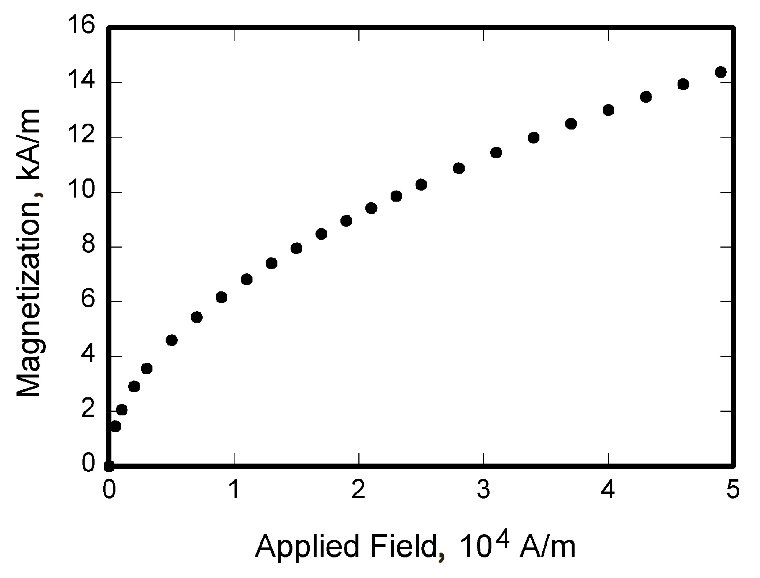
\includegraphics[width=1.0\textwidth]{Images/graph.jpg}
        \caption{graph 1}
        \label{subfig:graph1}
    \end{subfigure}
    \hfill
    \begin{subfigure}[t]{0.48\textwidth}
        \centering
        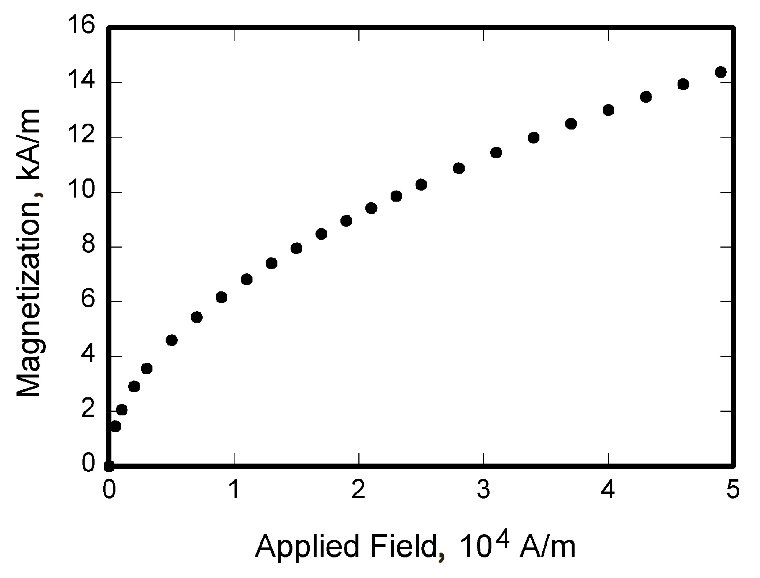
\includegraphics[width=1.0\textwidth]{Images/graph.jpg}
        \caption{graph 2}
        \label{subfig:graph2}
    \end{subfigure}
    \bigskip
    \begin{subfigure}[t]{0.48\textwidth}
        \centering
        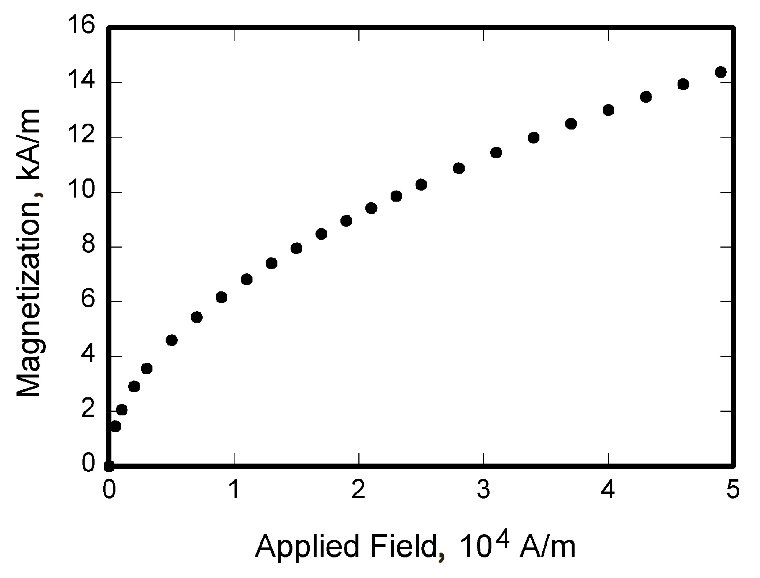
\includegraphics[width=1.0\textwidth]{Images/graph.jpg}
        \caption{graph 3 help help help help help help help help help help help help help}
        \label{subfig:graph3}
    \end{subfigure}
    \hfill
    \begin{subfigure}[t]{0.48\textwidth}
        \centering
        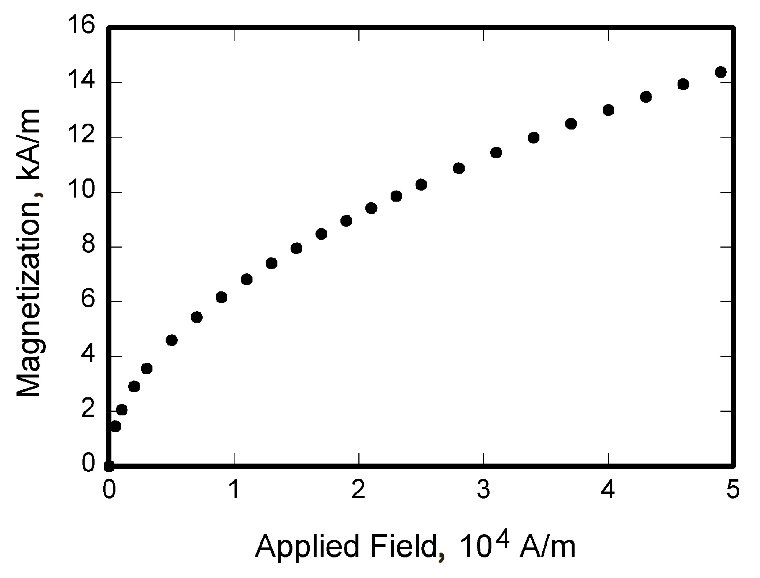
\includegraphics[width=1.0\textwidth]{Images/graph.jpg}
        \caption{graph 4}
        \label{subfig:graph4}
    \end{subfigure}
    \caption{graphs (subfigures)}
    \label{fig:graph_subfigures}
\end{figure}

\subsection{Continued float}
\begin{figure}[H]
    \centering
    \begin{subfigure}[t]{0.48\textwidth}
        \centering
        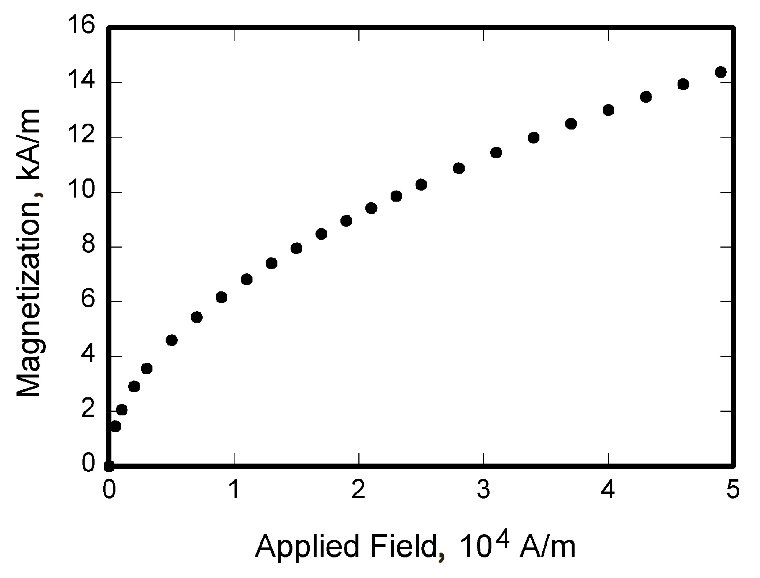
\includegraphics[width=1.0\textwidth]{Images/graph.jpg}
        \caption{graph 5}
        \label{subfig:graph5}
    \end{subfigure}
    \hfill
    \begin{subfigure}[t]{0.48\textwidth}
        \centering
        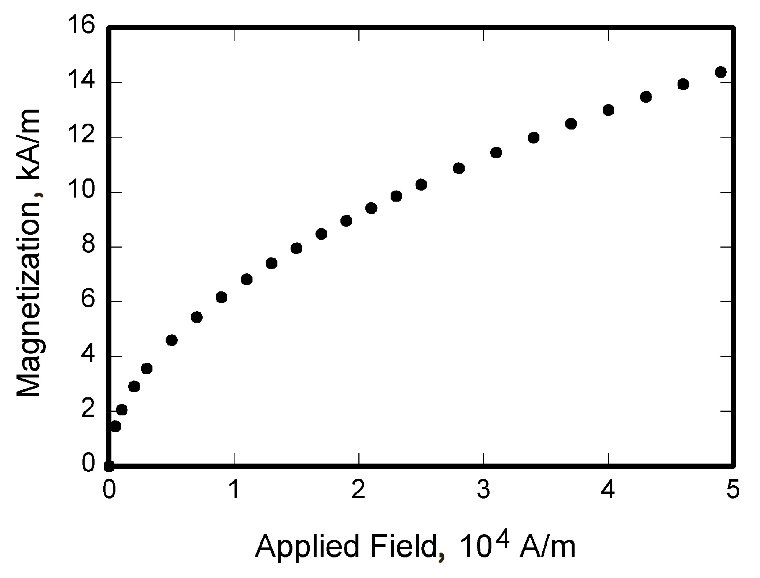
\includegraphics[width=1.0\textwidth]{Images/graph.jpg}
        \caption{graph 6}
        \label{subfig:graph6}
    \end{subfigure}
\end{figure}%
\begin{figure}[H]\ContinuedFloat
    \begin{subfigure}[t]{0.48\textwidth}
        \centering
        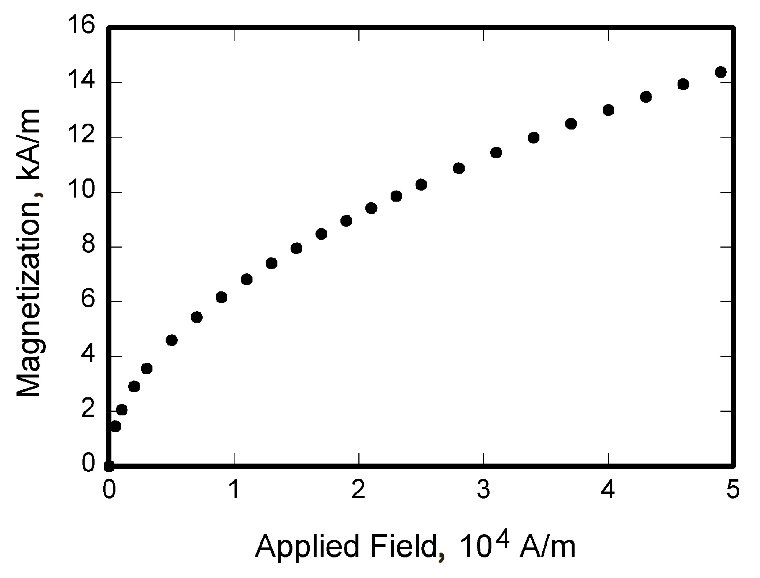
\includegraphics[width=1.0\textwidth]{Images/graph.jpg}
        \caption{graph 7}
        \label{subfig:graph7}
    \end{subfigure}
    \hfill
    \begin{subfigure}[t]{0.48\textwidth}
        \centering
        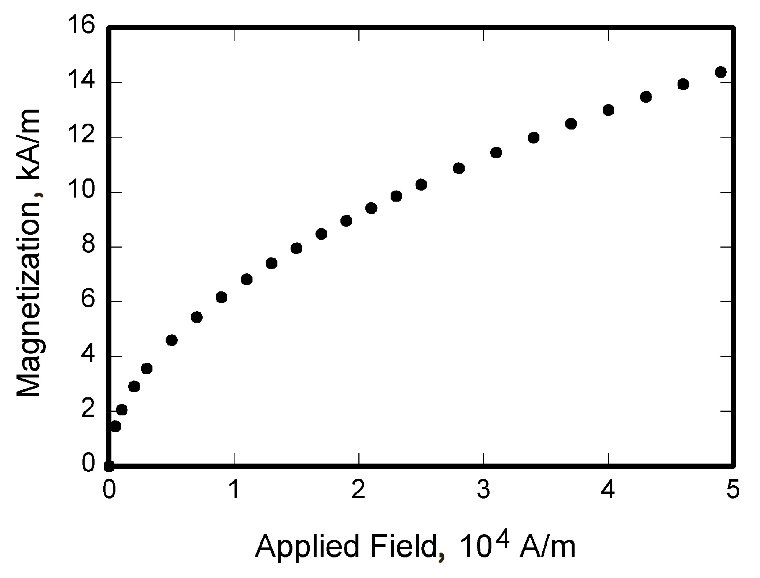
\includegraphics[width=1.0\textwidth]{Images/graph.jpg}
        \caption{graph 8}
        \label{subfig:graph8}
    \end{subfigure}
    \caption{graphs (continued float)}
    \label{fig:graph_contfloat}
\end{figure}

\DeclareRobustCommand{\VAN}[0]{van} % Change from Van to van
% \printbibliography[title={Works Cited}, heading=bibintoc]
\renewcommand{\bibname}{Works Cited}
%\begin{multicols}{2}[\printbibheading]
\printbibliography%[heading=none]
%\end{multicols}

%% If your highest level are chapters, then use this line!
\newcommand\invisibleappendix[1]{                % makes an invisible appendix header!
  \addcontentsline{toc}{chapter}{\protect{\thechapter}#1}%
  \chaptermark{#1}}
  
%% If your highest level are parts, then use this line below instead!
% \newcommand\invisibleappendix[1]{                % makes an invisible appendix header!
%   \addcontentsline{toc}{part}{\protect{\thechapter}#1}%
%   \chaptermark{#1}}

\renewcommand{\thesection}{\Alph{section}}
\renewcommand{\thesubsection}{\Alph{section}.\arabic{subsection}}
\renewcommand{\sectionmark}[1]{\markboth{#1}{}}
\renewcommand{\subsectionmark}[1]{\markright{#1}} % If this was not enabled in the main file.

\titleformat{\section}
  {\Large\bfseries}
  {{\fontfamily{qhv}\selectfont Appendix} \Huge{\thesection}\space}{5pt}{\fontfamily{qhv}\selectfont#1}[]
\titlespacing{\section}{0pt}{0.5\baselineskip}{0pt}

\titleformat{\subsection}
  {\bfseries}
  {\thesubsection\space}{5pt}{\fontfamily{qhv}\selectfont#1}[]
\titlespacing{\section}{0pt}{0.5\baselineskip}{0pt}

\newpage
\pagestyle{appendix}
\appendix
% \markboth{APPENDICES}{APPENDICES} % Solution to wrong header name provided in https://latex.org/forum/viewtopic.php?t=19574
\invisibleappendix{Appendices}

%%% GENERAL FORMAT OF APPENDICES:

% \section{TEST}
% \startcontents[sections]
% \printcontents[sections]{l}{1}[2]
% DESCRIPTOR

% \subsection{A}
% \subsection{B}

% \stopcontents[sections]

\section{Appendix First}
\label{app:AppendixFirst}

\startcontents[sections]
\printcontents[sections]{l}{1}[2]

blablablabla

\newpage

\invisiblesubsection{Appendix Second}
blabla





\stopcontents[sections]

\end{document}